\section{Evaluation}
\label{sec:evaluation}

We have applied our recurrent clustering algorithm to several scenarios, with mixed results. A major difficulty in evaluating these clusters is that we have no ``ground truth'', i.e. there is no objectively correct way to compare expressions. Instead, we provide a qualitative overview of the more interesting characteristics.

As a simple example, we clustered (Haskell equivalents of) the running examples used to present ACL2(ml) \citep{heras2013proof}, shown in Figure \ref{fig:lisp}. These include tail-recursive and non-tail-recursive implementations of several functions. We expect those with similar \emph{structure} to be clustered together, rather than those which implement the same function. The results are shown in Figure \ref{fig:haskellcluster}, where we can see the ``\hs{Tail}'' functions clearly distinguished, with little distinction between the tail recursive and na\"{\i}ve implementations.

Next we tested whether these same functions would be clustered together when mixed with seemingly-unrelated functions, in this case 207 functions from Haskell's \hs{text} library. In fact, the \hs{helperFib} and \hs{fibTail} functions appeared together in a separate cluster from the rest. This was unexpected, with no obvious semantic connection between these two functions and the others in their cluster (although most are recursive, due to the nature of the \hs{text} library).

\begin{figure}
  \begin{haskell}
(defun fact (n)
  (if (zp n) 1 (* n (fact (- n 1)))))

(defun helper-fact (n a)
  (if (zp n) a (helper-fact (- n 1) (* a n))))

(defun fact-tail (n)
  (helper-fact n 1))

(defun power (n)
  (if (zp n) 1 (* 2 (power (- n 1)))))

(defun helper-power (n a)
  (if (zp n) a (helper-power (- n 1) (+ a a))))

(defun power-tail (n)
  (helper-power n 1))

(defun fib (n)
  (if (zp n)
      0
      (if (equal n 1)
          1
          (+ (fib (- n 1)) (fib (- n 2))))))

(defun helper-fib (n j k)
  (if (zp n)
      j
      (if (equal n 1)
          k
          (helper-fib (- n 1) k (+ j k)))))

(defun fib-tail (n)
  (helper-fib n 0 1))
  \end{haskell}
  \caption{Common Lisp functions, both tail-recursive and non-tail-recursive.}
  \label{fig:lisp}
\end{figure}

\begin{figure}
  \begin{haskell}
fact n = if n == 0
            then 1
            else n * fact (n - 1)

helperFact n a = if n == 0
                    then a
                    else helperFact (n - 1) (a * n)

factTail n = helperFact n 1

power n = if n == 0
             then 1
             else 2 * power (n - 1)

helperPower n a = if n == 0
                     then a
                     else helperPower (n - 1) (a + a)

powerTail n = helperPower n 1

fib n = if n == 0
           then 0
           else if n == 1
                   then 1
                   else fib (n - 1) + fib (n - 2)

helperFib n j k = if n == 0
                     then j
                     else if n == 1
                          then k
                          else helperFib (n - 1) k (j + k)

fibTail n = helperFib n 0 1
  \end{haskell}
  \caption{Haskell equivalents of the Common Lisp functions in Figure \ref{fig:lisp}.}
  \label{fig:haskelllisp}
\end{figure}

\begin{figure}
  \centering
    \tikzstyle{block} = [rectangle, draw]
    \tikzstyle{line}  = [draw, -latex']
    \begin{tikzpicture}[node distance=3cm]
      \node [block] (c1) {
        \begin{tikzpicture}[node distance = 1cm]
          \node [block]                    (factTail)  {\hs{factTail}};
          \node [block, below of=factTail] (fibTail)   {\hs{fibTail}};
          \node [block, below of=fibTail]  (powerTail) {\hs{powerTail}};
        \end{tikzpicture}
      };
      \node [block, right of=c1] (c2) {
        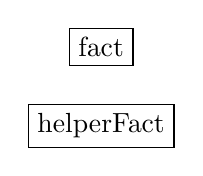
\begin{tikzpicture}[node distance = 1cm]
          \node [block]                (fact)       {\hs{fact}};
          \node [block, below of=fact] (helperFact) {\hs{helperFact}};
        \end{tikzpicture}
      };
      \node [block, right of=c2] (c3) {
        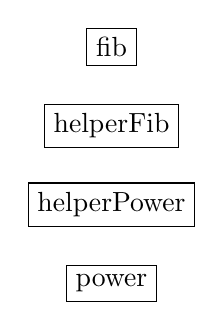
\begin{tikzpicture}[node distance = 1cm]
          \node [block]                       (fib)         {\hs{fib}};
          \node [block, below of=fib]         (helperFib)   {\hs{helperFib}};
          \node [block, below of=helperFib]   (helperPower) {\hs{helperPower}};
          \node [block, below of=helperPower] (power)       {\hs{power}};
        \end{tikzpicture}
      };
  \end{tikzpicture}
  \caption{Typical clusters for the functions in Figure \ref{fig:haskelllisp}.}
  \label{fig:haskellcluster}
\end{figure}

We have also applied our recurrent clustering algorithm to a variety of the most-downloaded packages from \textsc{Hackage} (as of 2015-10-30), including \texttt{text} (as above), \texttt{pandoc}, \texttt{attoparsec}, \texttt{scientific}, \texttt{yesod-core} and \texttt{blaze-html}. Whilst we expected functions with a similar purpose to appear together, such as the various reader and writer functions of \hs{pandoc}, there were always a few exceptions which became separate for reasons which are still unclear.

When clustering the \hs{yesod} Web framework, the clustering did seem to match our intuitions, in particular since all 15 of Yesod's MIME type identifiers appeared in the same cluster.

Whilst recurrent clustering has produced results which merit further investigation, the application to theory exploration has yet to be tested empirically. This is due to \qspec{}'s use of \qcheck{}'s \hs{Arbitrary} type class to generate random values for instantiating variables. Whilst we can automatically define \qspec{} theories and invoke them with \hs{nix-eval}, not all types have \hs{Arbitrary} instances; those without cannot be given any variables in our signature, which severely limits the possible combinations which can be explored. In many cases, no variables can be included at all, leaving just equations involving constants. This has so far prevented us from measuring the direct impact on \qspec{} performance, either directly by exploring the sub-sets identified through recurrent clustering, or indirectly by comparing the equations generated by a full brute-force search to our recurrent clusters: those equations relating terms from different clusters would not be discovered by our method. It is this ratio of equations found through brute force to those found after narrowing-down by clusters which is one of our key objectives to maximise at this stage; until we begin to pursue the \emph{interestingness} of the properties.

The following less-serious problems were also encountered while applying \textsc{ML4HS} to \textsc{Hackage} packages:

\begin{itemize}
  \item Some packages, such as \texttt{warp} and \texttt{conduits}, get no declarations to cluster. This is because they make all of their declarations privately, e.g. in ``internal'' modules, then use separate modules to export the public declarations. GHC's renaming phase makes all references to such exports canonical, by pointing them to the private declarations. This forces us to ignore such declarations, as \qspec{} will not be able to access them.

  \item Since we do not support type-level entities, we ignore type classes. Unfortunately, this also means ignoring any value-level bindings (AKA ``methods'') which occur in a type class instance. Instead of being clustered, these result in references getting $f_{recursion}$ features. This is especially noticable in libraries like \hs{scientific}, where only the functions for constructing and destructing numbers in scientific notation are clustered; all of the arithmetic is defined in type classes. One difficulty with supporting methods is that their namespace in Core is disjoint from that of regular Haskell identifiers: a transformation layer would be required, along with explicit type annotations to avoid ambiguity.
\end{itemize}

It seems like this recurrent clustering method has promise, although it will require a more thorough exploration of the parameters to obtain more intuitively reliable results. These clusters can then be used in several ways to perform theory exploration; the most na\"{\i}ve way being to explore each cluster as \qspec{} signature in its own right. \textsc{ML4HS} already provides this functionality, although the lack of test generators severely limits what can be discovered.

As alluded to previously, we also have the opportunity to reason by \emph{analogy}. Similar to the work on ACL2(ml) \citep{heras2013proof}, we could produce a general ``scheme'' from each equation we find (either through \qspec{} or by data mining test suites); like Isabelle approaches have shown \citep{Montano-Rivas.McCasland.Dixon.ea:2012}, these schemes could then be instantiated to a variety of similar values, in an attempt to find new theorems which are analogues of existing results from a different context. ``Mutating'' existing theorem statements in such a way would also increase the chance of any result being considered interesting; since it's likely that the unmodified statement was deemed interesting, and the new result would not in general follow as a simple logical consequence.
